%%%%%%%%%%%%%%%%%%%%%%%%%%%%%%%%%%%%%%%%%%%%%%%%%%%%%%%%%%%%%%%%%%%%%%%%%%%%%%%%
%	TRABAJO: Proyecto Integrador
%		Titulo: 	Desarrollo de IP cores con procesamiento de Redes de Petri 	
%					Temporales para sistemas multicore en FPGA					
%		Autores:	Juli�n Nonino												%					Carlos Renzo Pisetta										%		Director:	Orlando Micolini											
%%%%%%%%%%%%%%%%%%%%%%%%%%%%%%%%%%%%%%%%%%%%%%%%%%%%%%%%%%%%%%%%%%%%%%%%%%%%%%%%

% Path im�genes: ./marco_teorico/concurrencia/img
% Nombre predeterminado im�genes: concurrenciaxx
%	xx es el numero de imagen

\chapter{Concurrencia y Sincronizaci�n}
	\label{chap:chap_concurrencia}

	En los sistemas de computaci�n actuales conviven m�ltiples procesos que cooperan para lograr determinados objetivos y compiten por recursos del sistema, entre ellos el procesador, la memoria RAM, los puertos de entrada/salida, etc.
	
	Dado que generalmente el n�mero de procesos en un sistema supera ampliamente el n�mero de recursos, se deben establecer formas de comunicaci�n y sincronizaci�n entre ellos que hagan que el sistema funcione correctamente.

	En �ste capitulo se definir� cuando dos programas son concurrentes y/o paralelos y las condiciones que deben cumplirse para que dos secciones de c�digo fuente puedan ser ejecutadas de manera concurrente. Luego, se ver� que la ejecuci�n concurrente de procesos trae aparejados ciertos problemas como el interbloqueo y la inanici�n. Por esta raz�n deben utilizarse ciertos mecanismos de control para garantizar la correcta ejecuci�n de los programas, entre ellos, los sem�foros y los monitores.

	El objetivo de este cap�tulo es que el lector adquiera una idea general sobre la programaci�n concurrente y sobre los problemas inherentes a la misma.
	
	% Concurrencia
		%%%%%%%%%%%%%%%%%%%%%%%%%%%%%%%%%%%%%%%%%%%%%%%%%%%%%%%%%%%%%%%%%%%%%%%%%%%%%%%%%%%%%
%																					%
%	TRABAJO: Proyecto Integrador													%
%																					%
%		Titulo: 	Desarrollo de IP cores con procesamiento de Redes de Petri 		%
%					Temporales para sistemas multicore en FPGA						%
%																					%
%		Autores:	Juli�n Nonino													%
%					Carlos Renzo Pisetta											%
%		Director:	Orlando Micolini												%
%																					%
%	Parte: Marco Teorico															%
%	Capitulo: FPGA - IP cores - HDL													%
%	Seccion: Concurrencia y Paralelismo												%	
%	Archivo: concurrencia.tex														%
%																					%
%%%%%%%%%%%%%%%%%%%%%%%%%%%%%%%%%%%%%%%%%%%%%%%%%%%%%%%%%%%%%%%%%%%%%%%%%%%%%%%%%%%%%

% Path Imagenes: ./marco_teorico/concurrencia/img
% Nombre predeterminado imagenes: concurrenciaxx
%	xx es el numero de imagen

\section{Concurrencia y Paralelismo}
	\label{sec:concurrencia}

	Dos procesos ser�n concurrentes cuando la primera instrucci�n de uno de ellos se 
	ejecuta despu�s de la primera instrucci�n de otro proceso y antes de la �ltima. \cite{palma}
	
	No es necesario que se ejecuten al mismo tiempo, alcanza con el hecho de que se intercalen 
	sus instrucciones. En caso de ejecutarse al mismo tiempo se dice que hay programaci�n paralela.
	
	La programaci�n concurrente es un paralelismo potencial dependiente del hardware que lo soporte.
	
	\subsection{Condiciones de Bernstein}
		\label{subsec:condiciones_bernstein}
		
		No todas las partes de un programa pueden ejecutarse concurrentemente. Las condiciones de 
		Bernstein permiten determinar formalmente que partes de un programa pueden ejecutarse 
		concurrentemente y cuales no.
		\\ 
		
		Sean el conjunto de instrucciones $S_k$, pueden determinarse dos subconjuntos a partir de �l.
		\begin{itemize}
		  	\item $L(S_k) = \{a_1, a_2, \cdots, a_n\}$
		  		\\
				Subconjunto de $S_k$ que agrupa aquellas instrucciones que realizan lecturas de variables 
				durante la ejecuci�n del programa.
			\item $E(S_k) = \{b_1, b_2, \cdots , b_m\}$
				\\
				Subconjunto de $S_k$ que agrupa aquellas instrucciones que realizan escrituras de variables 
				durante la ejecuci�n del programa.
		\end{itemize}
		Luego, para que dos conjuntos de instrucciones $S_i$ y $S_j$ puedan ser ejecutadas de manera concurrente
		se deben cumplir las siguientes condiciones.
		\begin{equation*}
			\begin{array}{c}
				% Primera Fila
					L(S_i) \bigcap E(S_i) = \emptyset
				\\
				
				\\
				% Segunda Fila
					E(S_i) \bigcap L(S_i) = \emptyset
				\\
				
				\\
				% Tercera Fila
					E(S_i) \bigcap E(S_i) = \emptyset
			\end{array}
		\end{equation*}

	\subsection{Problemas inherentes a la programaci�n concurrente}
	
		La intercalaci�n de instrucciones de diferentes procesos, debe ser bien manejada y controlada 
		dado que puede producir mal funcionamiento del sistema. Los problemas inherentes a la 
		concurrencia son:
		\begin{itemize}
		  	\item \emph{Exclusi�n mutua}: Se debe garantizar que si un proceso adquiere el recurso los 
		  		dem�s deber�n esperar hasta que sea liberado.
		  	\item \emph{Condici�n de sincronizaci�n}: hay situaciones en las que un proceso debe esperar 
		  		que ocurra alg�n determinado evento para poder continuar. Por ello se debe garantizar que 
		  		si el evento NO ocurri�, el proceso NO contin�e.
		  	\item \emph{Interbloqueo}: Esta situaci�n se produce cuando todos los procesos est�n esperando 
		  		un evento que nunca ocurrir�. Se debe garantizar que estas situaciones no ocurran.
		  	\item \emph{Interbloqueo activo}: se produce cuando un sistema ejecuta una serie de instrucciones 
		  		sin hacer ning�n progreso.
		  	\item \emph{Inanici�n}: en este caso, el sistema en su conjunto hace progresos, pero existe un 
		  		grupo de procesos que nunca progresaran pues no se les otorga tiempo de procesador para hacerlo.
		\end{itemize}
				
	\subsection{Exclusi�n mutua}

		La \emph{exclusi�n mutua} implica que dos o m�s procesos intentan acceder a un �nico recurso o variable 
		compartida entre ellos pero solo uno puede acceder a cada instante.
		
		Cuando se da un caso de estas caracter�sticas, se desea que todo lo que necesite hacer uno de los procesos 
		sobre el recurso se realice de manera indivisible y luego lo deje disponible para que otro proceso ejecute 
		sus instrucciones sobre el recurso. La idea ser�a que instrucciones de diferentes procesos que act�en sobre 
		un mismo recurso NO sean intercaladas en la ejecuci�n.

		A la porci�n de c�digo que se desea que se ejecute de manera indivisible o at�mica se le llama \emph{secci�n 
		cr�tica}. Se debe lograr que todas las instrucciones dentro de la secci�n critica se ejecuten en exclusi�n 
		mutua lo que implica que el hecho de que cuando uno de los procesos este ejecutando esa porci�n de c�digo 
		el resto no podr� hacerlo.
		
		\textbf{\emph{SOLO UNO de los procesos podr� estar en la secci�n cr�tica en un instante dado.}}
		
		\begin{figure}[H]
			\centering
			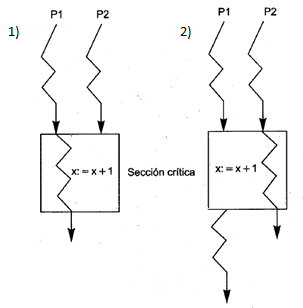
\includegraphics[width=0.6\linewidth,keepaspectratio]{./marco_teorico/concurrencia/img/concurrencia01}
			\caption{Secci�n cr�tica}
			\label{fig:concurrencia01}
		\end{figure}
		
		En la Figura \ref{fig:concurrencia01} se observa como dos procesos \emph{P1} y \emph{P2} intentan ejecutar 
		una porci�n de c�digo de una secci�n cr�tica. La imagen de la izquierda (1) muestra que el proceso \emph{P1} 
		consigue ingresar a ejecutar la secci�n critica. La imagen de la derecha (2) muestra que el proceso \emph{P2} 
		puede ingresar solo cuando el proceso \emph{P1} ya no esta en la misma.
		\\
		
		La exclusi�n mutua puede representarse con una Red de Petri de la siguiente manera.
		\begin{figure}[H]
			\centering
			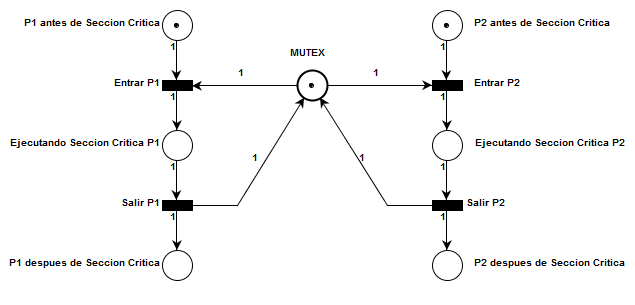
\includegraphics[width=1\linewidth,keepaspectratio]{./marco_teorico/concurrencia/img/concurrencia02}
			\caption{Exclusi�n mutua modelada con una Red de Petri}
			\label{fig:concurrencia02}
		\end{figure}
		En la Red de Petri de la Figura \ref{fig:concurrencia02} se representa una situaci�n de exclusi�n mutua. 
		La plaza \emph{MUTEX} esta limitada a un �nico token y el an�lisis de invariantes de plazas demuestra 
		formalmente la propiedad de exclusi�n mutua entre los procesos \emph{P1} y \emph{P2}.
		\begin{equation*}
			m(EjecutandoSCP1) + m(MUTEX) + m(EjecutandoSCP2) = 1
		\end{equation*}
		
	\subsection{Condici�n de sincronizaci�n}
	
		Existen situaciones en las que un recurso compartido por varios procesos se encuentra en un estado en el 
		que un proceso no puede hacer una determinada acci�n con el hasta que no cambie el estado. A esto se llama 
		\emph{condici�n de sincronizaci�n}.
		
		Por ello se debe contar con mecanismos que permitan bloquear a un proceso que no pueda hacer algo en un 
		momento determinado a la espera de alg�n evento. Pero tambi�n, mecanismos que permitan desbloquearlo 
		cuando el evento haya ocurrido.
		
	\subsection{Propiedades de los programas concurrentes}
		
		Para que un programa sea correcto debe cumplir las especificaciones funcionales. En el caso de los programas 
		concurrentes deben, adem�s, cumplir con una serie de propiedades inherentes a la concurrencia.
		Estas propiedades se agrupan en:
		\begin{itemize}
		  	\item \emph{Propiedades de seguridad}: aseguran que nada malo va a pasar durante la ejecuci�n del programa.
		  	\item \emph{Propiedades de vivacidad}: aseguran que algo bueno pasara eventualmente durante la ejecuci�n.
		\end{itemize}
	
		\subsubsection{Propiedades de seguridad}
			
			\begin{itemize}
			  	\item \emph{Exclusi�n mutua}: dado que existen recursos en el sistema que deben ser accedidos en exclusi�n 
			  		mutua, se debe garantizar que si un proceso adquiere el recurso los dem�s deber�n esperar hasta que sea 
			  		liberado.
			  	\item \emph{Condici�n de sincronizaci�n}: en las situaciones en las que un proceso debe esperar que ocurra 
			  		alg�n determinado evento para poder continuar, se debe garantizar que si el evento NO ocurri�, el proceso 
			  		NO contin�e.
			  	\item \emph{Interbloqueo}: Esta situaci�n se produce cuando todos los procesos est�n esperando un evento que 
			  		nunca ocurrir�. Se debe garantizar que estas situaciones no ocurran. Tambi�n se conoce con el nombre de 
			  		\textbf{\emph{deadlock}}.
			\end{itemize}
		
		\subsubsection{Propiedades de vivacidad}
			
			\begin{itemize}
			  	\item \emph{Interbloqueo activo}: se produce cuando un sistema ejecuta una serie de instrucciones sin hacer 
			  		ning�n progreso. Se conoce como \textbf{\emph{livelock}}.
			  	\item \emph{Inanici�n}: en este caso, el sistema en su conjunto hace progresos, pero existe un grupo de 
			  		procesos que nunca progresaran pues no se les otorga tiempo de procesador para hacerlo. Tambi�n se 
			  		conoce como \textbf{\emph{starvation}}. 
			\end{itemize}
	
		\subsubsection{Ejemplo}
		
			El siguiente ejemplo ha sido extra�do de \cite{palma} e ilustra todos los problemas antes mencionados.
			\\
			
			Sea un juego donde hay dos equipos, el \emph{A} y el \emph{B}, y un juez con un pa�uelo.
			Cada jugador de un equipo tiene un n�mero del \emph{1} al \emph{3}. No puede haber jugadores del mismo 
			equipo con el mismo n�mero.
			
			El juez dice un n�mero y los dos rivales con el mismo n�mero van corriendo a buscar el pa�uelo. El que 
			lo agarre debe volver a su lugar sin que su rival le toque la espalda.

			A continuaci�n se describir�n, para �ste ejemplo, las propiedades mencionadas anteriormente.
			\begin{itemize}
			  	\item \emph{Exclusi�n mutua}: al pa�uelo puede agarrarlo solo un jugador a la vez, si lo agarran dos 
			  		puede romperse, lo que implicar�a un mal funcionamiento del sistema.
				\item \emph{Condici�n de sincronizaci�n}: un jugador debe esperar a que digan su n�mero para correr.
				\item \emph{Interbloqueo}: si un jugador se guarda el pa�uelo y se va. El juez esperar�a que se lo 
					devuelvan y los jugadores que el juez diga su nombre, pero ninguno de los eventos ocurrir�.
				\item \emph{Interbloqueo activo}: se producir�a si dos jugadores amenazan una y otra vez con agarrar 
					el pa�uelo pero ninguno lo hace.
				\item \emph{Inanici�n}: Podr�a pasar si el juez nunca dice el nombre de un jugador en particular.
			\end{itemize}
	
	\subsection{Interbloqueo}
		
		En un sistema donde los procesos compiten por limitados recursos, pueden producirse demandas contradictorias 
		de los mismos. Por ejemplo, si existen dos procesos, \emph{A} y \emph{B}, y dos recursos, \emph{R1} y \emph{R2}, 
		y ambos procesos necesitan los dos recursos para proseguir, si el proceso \emph{A} toma el recurso \emph{R1} y 
		el \emph{B} el recurso \emph{R2}, ambos procesos se bloquearan a la espera del otro recurso, pero ninguno liberara 
		el recuro que posee hasta no conseguir los dos. A esta situaci�n se la conoce como interbloqueo. \cite{stallings}
		
		\subsubsection{Condiciones para producir interbloqueo}
		
			El interbloqueo podr� producirse si se cumplen tres condiciones:
			\begin{enumerate}
			  	\item \emph{Exclusi�n mutua}: s�lo un proceso puede utilizar el recurso en un momento determinado.
			  	\item \emph{Retenci�n y espera}: un proceso puede mantener el recurso que se le asigno mientras espera 
			  		conseguir otro.
			  	\item \emph{No apropiaci�n}: ning�n proceso podr� ser forzado a abandonar un recurso que retiene.
			  	\item \emph{Circulo viciosos de espera}: Existe una cadena cerrada de procesos donde cada proceso retiene 
			  		un recurso que necesita un proceso que le sigue en la cadena.
			\end{enumerate}

			Las tres primeras condiciones son necesarias pero no suficientes para que se produzca interbloqueo.
			
			La cuarta es una consecuencia potencial de las tres primeras y, en caso de darse, generar� un \textbf{\emph{c�rculo 
			vicioso de espera irresoluble}}.
			
			Un c�rculo de espera irresoluble es la definici�n de interbloqueo.
				
		\subsubsection{Prevenci�n del interbloqueo}
			
			La idea es intentar dise�ar un sistema donde, la posibilidad de interbloqueo este excluida.
			\newpage
			Existen dos tipos de m�todos para internar prevenir una situaci�n de interbloqueo:
			\begin{itemize}
			  	\item \emph{Indirectos:} intentan impedir la aparici�n de las tres condiciones necesarias (1,2 y 3).
			  	\item \emph{Directos}: intentan evitar la aparici�n de un c�rculo vicioso de espera irresoluble.
			\end{itemize}
		
			Existen diversas t�cnicas de prevenci�n de interbloqueo relacionadas a cada una de las condiciones que 
			pueden producirlo.
			\begin{itemize}
			  	\item \emph{Exclusi�n mutua}: En general no puede anularse, si un recurso necesita ser accedido en 
			  		exclusi�n mutua no podr� hacerse un acceso de sin esta condici�n.
			  	\item \emph{Retenci�n y espera}: esta condici�n puede prevenirse haciendo que todos los procesos 
			  		soliciten todos los recursos que necesitan al mismo tiempo y bloqueando al proceso hasta que 
			  		todos los recursos que necesite est�n disponibles simult�neamente. Pero esta soluci�n es 
			  		ineficiente por dos factores:
			  		\begin{itemize}
			  		  	\item Un proceso puede estar suspendido durante mucho tiempo esperando todos los recursos 
			  		  		cuando podr�a haber avanzado con algunos de ellos.
			  		  	\item Los recursos asignados a un proceso pueden permanecer mucho tiempo sin usarse. En ese 
			  		  		tiempo otro proceso podr�a haberlos utilizado.
			  		\end{itemize}
			  	\item \emph{No apropiaci�n}: puede prevenirse de varias maneras:
			  		\begin{itemize}
			  		  	\item Si un proceso que retiene muchos recursos pide uno m�s y se le niega el pedido, se le 
			  		  		obligara a liberar todos los recursos anteriores y volver a pedirlos cuando los necesite 
			  		  		junto con el recurso adicional.
			  		  	\item Si un proceso pide recursos retenidos por otro proceso, el sistema operativo puede 
			  		  		expulsar al segundo proceso y exigirle que libere sus recursos. Este sistema evitara 
			  		  		interbloqueo solo si existen dos procesos con la misma prioridad.
			  		\end{itemize}
			  	\item \emph{C�rculo vicioso de espera}: esta condici�n puede prevenirse definiendo un ordenamiento lineal 
			  		de los tipos de recursos. Por ejemplo si un proceso solicit� recursos del tipo \emph{R}, solo podr� 
			  		realizar peticiones posteriores sobre recursos siguientes a \emph{R} en el ordenamiento. Esta t�cnica 
			  		puede ser ineficiente porque se puede retardar procesos deneg�ndoles recursos innecesariamente. 
			\end{itemize}
			
		\subsubsection{Predicci�n del interbloqueo}
		
			En la prevenci�n del interbloqueo se obligaba a impedir que sucedieran algunas de las cuatro condiciones que 
			pueden llevar al interbloqueo. Pero con esto, se llega a un uso ineficiente de los recursos y a una ejecuci�n 
			ineficiente de los procesos.
			
			En cambio, en la predicci�n, se permiten alcanzar las tres condiciones necesarias pero se realizan elecciones 
			acertadas para evitar llegar al punto del interbloqueo. Por lo tanto, la predicci�n permite m�s concurrencia 
			que la prevenci�n.
			
			Con predicci�n de interbloqueo, antes de concederle un recurso a un proceso, se decidir� din�micamente si esa 
			petici�n puede llevar a interbloqueo en caso de concederse. Por lo tanto, la predicci�n exige saber las peticiones 
			futuras de recursos.

			Elementos de la predicci�n del interbloqueo son:
			\begin{itemize}
			  	\item \emph{Negativa de iniciaci�n de procesos}: no se iniciara un proceso si sus demandas pueden llevar a un 
			  		interbloqueo. Un nuevo proceso comenzara solo si puede satisfacerse la demanda m�xima de todos los procesos 
			  		actuales m�s la del nuevo proceso. Esta estrategia no es �ptima ya que asume el peor caso, que todos los 
			  		procesos expresen su mayor demanda al mismo tiempo.
			  	\item \emph{Negativa de asignaci�n de recursos}: no se conceder� una solicitud de incrementar los recursos de un 
			  	proceso si esta petici�n puede llevar a interbloqueo. Esta estrategia fue enunciada por Dijkstra y se conoce como 
			  	\textbf{\emph{algoritmo del banquero}}.
			\end{itemize}
			
		\subsubsection{Algoritmo del banquero}

			Este algoritmo comienza definiendo un estado seguro, donde existe al menos un orden en el cual todos los procesos 
			pueden ejecutar hasta el final sin producir interbloqueo. Un estado inseguro es, naturalmente, un estado no seguro.
			
			Cuando un proceso realiza un petici�n de recursos, se supone que se concede, se actualiza el estado del sistema, 
			si es seguro se concede la solicitud, en caso contrario se bloquea el proceso hasta que sea seguro conceder la 
			solicitud.
			
			El algoritmo es conocido de esta manera por analog�a con el problema de un banco cuando los clientes desean obtener 
			dinero prestado. Los clientes ser�an los procesos y el dinero los recursos. De esta manera, el banco tiene una 
			reserva limitada de dinero para prestar y un conjunto de clientes. Si un cliente pide un pr�stamo, el banquero 
			puede optar por rechazarlo si existe riesgo de que el banco se quede sin fondos suficientes para pr�stamos futuros.

			Como se observa, se debe conocer la m�xima solicitud por anticipado, los procesos deben ser independientes y el 
			n�mero de recursos y procesos debe ser fijo.
	

		
	% Sincronizaci�n
		%%%%%%%%%%%%%%%%%%%%%%%%%%%%%%%%%%%%%%%%%%%%%%%%%%%%%%%%%%%%%%%%%%%%%%%%%%%%%%%%
%	TRABAJO: Proyecto Integrador
%		Titulo: 	Desarrollo de IP cores con procesamiento de Redes de Petri 	
%					Temporales para sistemas multicore en FPGA					
%		Autores:	Juli�n Nonino												%					Carlos Renzo Pisetta										%		Director:	Orlando Micolini											
%%%%%%%%%%%%%%%%%%%%%%%%%%%%%%%%%%%%%%%%%%%%%%%%%%%%%%%%%%%%%%%%%%%%%%%%%%%%%%%%

% Path im�genes: ./marco_teorico/concurrencia/img
% Nombre predeterminado im�genes: concurrenciaxx
%	xx es el numero de imagen

\section{Sincronizaci�n}
	\label{sec:sincronizacion}

	Para solucionar los problemas inherentes a la programaci�n concurrente, se utiliza lo que se llama \emph{sincronizaci�n entre los procesos}.

	En general, se habla de sincronizaci�n cuando determinados fen�menos ocurren o deben ocurrir en un determinado orden o a la vez.

	Para la Ingenier�a en Computaci�n, la sincronizaci�n es representada por las se�ales que se env�an los procesos para colaborar entre ellos o para indicar el estado de recursos compartidos, para indicar que un evento o acci�n ocurri� o no y determinar si un proceso puede continuar o no, etc�tera.

	Se dice que un recurso esta sincronizado cuando debe encontrarse en un estado determinado para que un proceso pueda utilizarlo. En otras palabras, se puede definir a la condici�n de sincronizaci�n como a la propiedad requerida de que un proceso no realice ninguna acci�n o evento hasta que otro proceso realice una determinada acci�n o evento.
	
	Existen diversos mecanismos que se utilizan para sincronizar procesos, entre ellos, los m�s comunes son los \textbf{\emph{sem�foros}} y los \textbf{\emph{monitores}}.

	\subsection{Sem�foros}
	
		Los sem�foros son un sistema de se�ales simples utilizadas por los procesos para comunicarse entre ellos y lograr la sincronizaci�n requerida.

		En este m�todo se tiene una variable de sincronizaci�n, del tipo entero no negativo, que indica la cantidad de recursos disponibles. Sobre esta variable se realizan dos tipos de operaciones:
		\begin{itemize}
		  	\item \emph{wait}: decrementa el valor del sem�foro solo si este es mayor que cero. Este proceso indica que se utiliza uno de los recursos que controla el sem�foro. Si el valor del sem�foro al momento de ejecutar la operaci�n \emph{wait} es cero, indica que no hay recursos disponibles y el proceso debe bloquearse hasta que se libere alguno.  
		  	\item \emph{signal}: es la acci�n de liberar un recurso que estaba siendo usado por otro proceso en el sem�foro. En caso de haber alg�n proceso bloqueado en el sem�foro se lo despierta para que utilice el recurso. De no existir ning�n proceso, se incrementa el valor del sem�foro. 	
		\end{itemize}
		\begin{figure}[H]
			\centering
			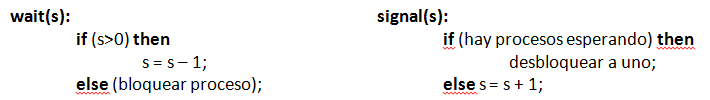
\includegraphics[width=1\linewidth,keepaspectratio]{./marco_teorico/concurrencia/img/concurrencia03}
			\caption{Operaciones \emph{wait} y \emph{signal} sobre un sem�foro \emph{s}}
			\label{fig:concurrencia03}
		\end{figure}
		
		Aunque los sem�foros son un mecanismo de gran potencia, se pueden enunciar los siguientes inconvenientes al usarlos.
		\begin{enumerate}
		  	\item Es un mecanismo de bajo nivel, no estructurado, que f�cilmente puede llevar a errores transitorios. La ejecuci�n de cada secci�n cr�tica debe comenzar con un \emph{wait} y terminar con un \emph{signal} sobre el mismo sem�foro. Si se omite una de estas operaciones o se realizan sobre sem�foros diferentes puede derivar en un mal funcionamiento del sistema, como por ejemplo, no garantizar exclusi�n mutua en las secciones cr�ticas.
		  	\item No se puede restringir el tipo de operaciones realizadas sobre los recursos.
		  	\item Cuando se usan sem�foros, el programador puede olvidar incluir en alguna secci�n cr�tica todas las sentencias necesarias para el control de los objetos compartidos.
		  	\item Tanto la exclusi�n mutua como la condici�n de sincronizaci�n se implementan de la misma manera. Esto hace dif�cil, al ver un \emph{wait} o un \emph{signal}, discernir acerca del prop�sito con el que fueron incluidas. Como la exclusi�n mutua y la condici�n de sincronizaci�n son conceptos distintos se desear�a que tengan notaciones diferentes.
		  	\item Los programas que utilizan sem�foros son muy dif�ciles de mantener dado que el c�digo de sincronizaci�n est� repartido entre los distintos procesos. Por lo tanto cada vez que se realiza una modificaci�n hay que revisar cada proceso.
		\end{enumerate}

	\subsection{Monitores}
		
		Como se dijo, los sem�foros, generalmente se encuentran dispersos en el c�digo, lo que lo hace m�s confuso y muchas veces es dif�cil notar cual es el recurso compartido y determinar si est� correctamente sincronizado. Por ello, se necesita un sistema que sea igual de vers�til que los sem�foros pero que permita efectuar un control m�s estructurado de la exclusi�n mutua. Una herramienta con estas caracter�sticas fue propuesta por \emph{C. A. R. Hoare} en 1975 y es llamada \textbf{\emph{monitor}}.

		Un \emph{monitor} es un mecanismo de abstracci�n de datos, lo que permite representar de forma abstracta un recurso compartido mediante variables que indican su estado. El acceso a esas variables solo es posible a trav�s de un conjunto de funciones/m�todos que el monitor exporta al exterior.
		
		Al usar monitores en la sincronizaci�n y en la exclusi�n mutua, existen dos clases de procesos:
		\begin{itemize}
		  	\item \emph{Procesos Pasivos}: son los que implementan los monitores y quedan a la espera que un proceso activo ejecute los m�todos exportados por el monitor.
		  	\item \emph{Procesos Activos}: son aquellos procesos que en un momento determinado pueden requerir utilizar el recurso controlado por el monitor para lo cual llaman a los m�todos que �ste exporta. 
		\end{itemize}

		Dado que las variables compartidas se encuentran dentro del monitor, los procesos activos solo pueden utilizarlas mediante los m�todos que el monitor exporta. Las ventajas de esto son dos:
		\begin{enumerate}
		  	\item Los programadores de los procesos activos no deben preocuparse de c�mo esta implementado el recurso compartido, es m�s, si se mantienen los nombres de los procedimientos exportados, esta implementaci�n puede cambiar sin necesidad de modificar a los procesos activos.
		  	\item El programador del monitor no se debe preocupar en c�mo y donde ser� utilizado el monitor, ya que una vez que se comprob� que el monitor funciona correctamente, seguir� funcionando de forma correcta en diferentes contextos.
		\end{enumerate}


		Un monitor se compone de los siguientes elementos:
		\begin{itemize}
		  	\item Un \emph{conjunto de variables} locales que pueden denominarse permanentes. Se utilizan para almacenar el estado interno del recurso que representa el monitor. Se denominan permanentes ya que permaneces sin modificarse entre dos llamadas consecutivas al monitor y solo pueden ser accedidas dentro del mismo.
		  	\item Un \emph{c�digo de inicializaci�n} que se ejecuta antes que la primera instrucci�n ejecutable del programa y su fin es inicializar las variables permanentes.
		  	\item Un \emph{conjunto de procedimientos internos} que manipulan las variables permanentes.
		  	\item Una \emph{declaraci�n de los procedimientos que son exportados} y pueden ser accedidos por los procesos activos externos.
		\end{itemize}
				
		\subsubsection{Exclusi�n mutua en monitores}
			
			El control de la exclusi�n mutua en un monitor se basa en la existencia de una cola asociada al mismo que se denominara \emph{cola del monitor}. La gesti�n de esta cola se realiza de la siguiente manera:
			\begin{enumerate}
			  	\item Cuando un proceso activo est� dentro del monitor (ejecutando alguno de los procedimientos del mismo) y aparece otro proceso activo que intenta ejecutar otro (o el mismo) procedimiento, el c�digo de acceso al monitor bloquea el proceso que realiza la llamada y lo inserta en la cola del monitor (con pol�tica FIFO). As�, se impide que dos procesos est�n al mismo tiempo dentro del monitor.
			  	\item Cuando un proceso activo abandona el monitor, este �ltimo selecciona el proceso que est� al frente de la cola del monitor y lo desbloquea para que comience a ejecutar las operaciones que le solicit� al monitor. Si la cola estaba vac�a, el monitor queda libre y cualquier proceso activo que llame alguno de sus procedimientos entrar� al monitor. 
			\end{enumerate}

			Esto asegura que las variables compartidas nunca son accedidas concurrentemente. Una cuesti�n importante es que la responsabilidad de bloquear un proceso es del monitor y no del proceso. 
			
			Al comparar este sistema con un sem�foro se ve que en el caso de los sem�foros son los propios procesos activos los que manejan las pol�ticas de acceso a variables compartidas.
			
		\subsubsection{Condici�n de sincronizaci�n en monitores}
		
			Para que un monitor pueda controlar condiciones de sincronizaci�n, se utilizan las llamadas variables de condici�n que se declaran dentro del monitor. Los valores de estas variables no son accesibles por el programador y representan colas FIFO. Estas variables permiten bloquear un proceso que no puede seguir su ejecuci�n dentro de monitor y desbloquearlos cuando la situaci�n que provoco el bloqueo ya no se est� presente. Para conseguir esto se necesitan dos operaciones sobre las variables de condici�n. Las operaciones \textbf{\emph{delay}} y \textbf{\emph{resume}}. La operaci�n \emph{delay(C)}, siendo \emph{C} una variable de condici�n, hace que el proceso se bloquee en la cola asociada a dicha variable. Hay que remarcar que el proceso no puede bloquearse directamente, antes de bloquearse al final de la cola de la condici�n debe liberar la exclusi�n mutua que retiene sobre el monitor. Si un proceso ha sido bloqueado con la operaci�n \emph{delay(C)} solo puede ser desbloqueado con la operaci�n \emph{resume(C)}. Esta �ltima operaci�n despierta al proceso que est� al frente de la cola de la condici�n y lo prepara para su ejecuci�n. Si la cola estaba vac�a se transforma en una operaci�n nula.

			Con lo dicho hasta este punto, se podr�a decir que si un proceso que se est� ejecutando dentro del monitor ejecuta una operaci�n \emph{resume(C)}, se desbloquear� un proceso de esa cola que continuar� con su ejecuci�n dentro del monitor tambi�n. Esto lleva a una situaci�n con dos procesos dentro del monitor, lo que violar�a la exclusi�n mutua. Para evitar esto, el proceso que ejecuta el \emph{resume} ceder� cort�smente la exclusi�n mutua al reci�n desbloqueado. Y espera en una cola diferente llamada \textbf{\emph{cola de cortes�a}} hasta que el proceso reci�n desbloqueado por el \emph{resume(C)} termine su ejecuci�n teniendo preferencia por sobre los procesos esperando en otras colas.
		
	\subsection{Implementaci�n de monitores con Redes de Petri}
	
		Es posible ver a un monitor formado por dos secciones: primero, la referida a la pol�tica de colas que se debe ejecutar para lograr que s�lo un proceso est� en el monitor, que se bloqueen los procesos que no tienen los recursos y que se desbloqueen los que obtuvieron los recursos, y segundo, la l�gica con que se administran los recursos.

		En la Figura \ref{fig:concurrencia04} se puede observar que existe una cola de entrada, para los procesos que a�n no ingresaron al monitor y desean hacerlo, una serie de colas, una por cada recurso (cada condici�n de sincronizaci�n) y una cola de cortes�a para que el proceso dentro del monitor pueda, de manera segura, ceder la exclusi�n mutua al cambiar el estado de un recurso.

		\textbf{\emph{Una Red de Petri puede realizar el trabajo de la l�gica del monitor}}, es decir, controlar la exclusi�n mutua y/o la administraci�n de recursos disponibles; esto es cuando el vector de estado que result� del disparo no tiene componentes negativas es porque los recursos est�n disponibles, el disparo de la transici�n solicitada conduce a un nuevo estado valido. De no ser as�, en caso de existir alg�n valor negativo en el nuevo vector de estado, se lleg� a un estado no v�lido que indica que el recurso no est� disponible. Adem�s el vector de estado indica si el disparo ha devuelto o tomado recursos. Si la cantidad de tokens para un recurso dado disminuye, significa que se han tomado recursos, en caso contrario, que se han devuelto recursos.
		\begin{figure}[H]
			\centering
			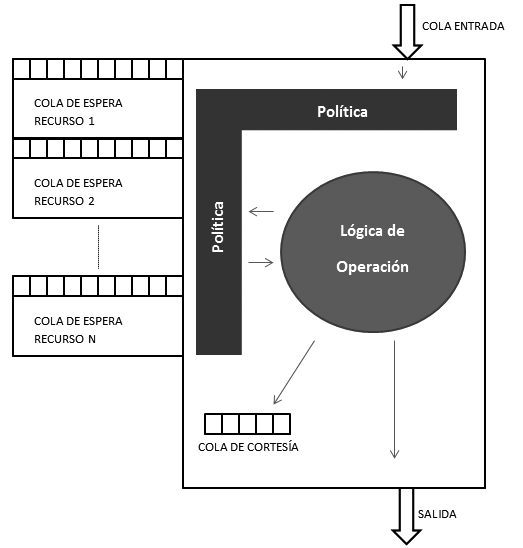
\includegraphics[width=1\linewidth,keepaspectratio]{./marco_teorico/concurrencia/img/concurrencia04}
			\caption{Monitor}
			\label{fig:concurrencia04}
		\end{figure}
		